\documentclass[../3Wworkreport.tex]{subfiles}
\doublespacing
%\setcounter{section}{0}
\pagenumbering{arabic}

\begin{document}
\section{Introduction}
\label{sec:intro}

Quantum computing has made great strides in recent years, and is emerging as a popular field for mathematicians, physicists, computer scientists, and electrical engineers. From a theoretical standpoint, developing algorithms that take advantage of quantum phenomena and characterizing the differences between quantum and classical computational algorithms is necessary to determine precisely what resources are needed for quantum computers to be more effective than current computers. The quantum bit (qubit) is a basis for much of the theoretical framework of quantum computing, and its two-state design is analogous to the 0-1 framework of classical computers. Working in dimensions higher than two (qubits are renamed qudits to emphasize the $d$-dimensional systems) can yield some results that are more intuitive than results found in two dimensions.\\

One area of study in quantum computing is communication complexity, and how entangled particles can help physically separated parties perform calculations. Given a problem, the communication complexity is the minimum amount of information exchanged between the two parties needed to solve the problem \parencite{kushilevitz2006}. Examining the information that must be exchanged between parties has ties to cryptography, secure communication channels, and distributed computation.\\

Another relevant topic of interest is known as the stabilizer sub-theory. It involves certain quantum operators (also called gates, which are mathematically represented by unitary matrices) and how quantum algorithms associated with these operators can be simulated efficiently on classical computers. Closely related to the formalism of stabilizers is the discrete Wigner function, which serves as both an intuitive approach to quantum states and a mathematical representation of them. As both of these areas are quite technical, the reader should refer to \Cref{app:stabilizer,app:dwf} for a better understanding of these topics.\\

While communication complexity and the stabilizer sub-theory are not highly related topics, some problems arising from a communication complexity framework can be solved effectively by developing algorithms that are based upon the stabilizer formalism. One such problem is known as Raz's problem.\\

Raz's problem \parencite{Raz1999} comes in two variants, but both are based off of the same premise. The following definitions are consistent across both variants: the two parties of interest are named Alice and Bob; $x \in \mathbb{R}^d$ is a unit vector, where $d$ is an odd prime number; $M_0$ and $M_1$ are orthogonal subspaces of $\mathbb{R}^d$; and $\vartheta \in \mathbb{R}$ where $0 \le \vartheta < 1/\sqrt{2}$.
\begin{prob}
Let Alice have the vector $x$, Bob have the subspaces $M_0$ and $M_1$, and both Alice and Bob have the value $\vartheta$. Alice and Bob must communicate to output the value 0 if the distance d($x,M_0) < \vartheta$, and 1 otherwise.
\end{prob}

\begin{prob}
Let Alice have $x$ and the subspaces $M_0, M_1$, Bob have an orthogonal matrix $U$, and both Alice and Bob have the value $\vartheta$. Alice and Bob must communicate to output the value 0 if the distance d($Ux,M_0) < \vartheta$, and 1 otherwise.
\end{prob}

The goal is to provide solutions to these problems that minimize the communication complexity between Alice and Bob. A visual representation of these problems can be seen in \Cref{fig:razproblem}. Raz showed that there exists a protocol which solves Problem 2 where the lower bound for its complexity, using probabilistic classical computation, is $\Omega(\sqrt{d})$, and the upper bound is $O(d^{3/4})$ \parencite{Raz1999}. There is also a bound for Problem 1 of $O(\sqrt{d})$. As stated by Raz, and further discussed by Buhrman et al., efficient quantum computational protocols, however, have a communication complexity of $\Theta(log\,d)$, demonstrating an exponential separation in complexity between the two methods \parencite{Buhrman2009}. The purpose of this report, then, is to develop a classical protocol that  behaves like the quantum protocols in special cases, and approaches the classical lower bounds in general. In addition, the report characterizes the special cases and how the protocols behaves in general.

\begin{figure}[!h]
\begin{center}
\subfloat[Raz's Problem 1]{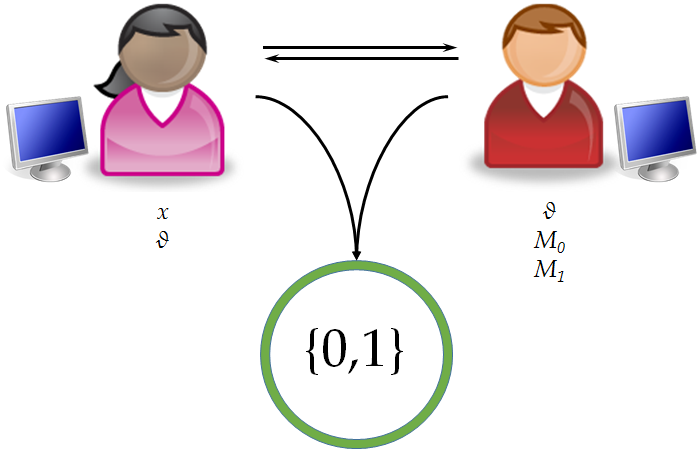
\includegraphics[width=0.5\textwidth]{Raz_prob1.png}}
\subfloat[Raz's Problem 2]{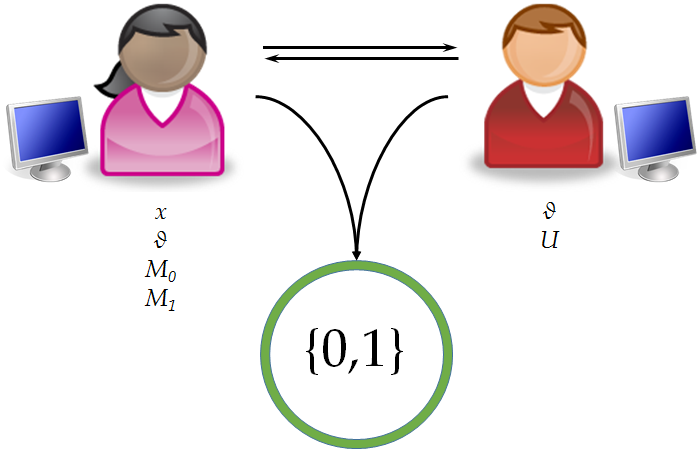
\includegraphics[width=0.5\textwidth]{Raz_prob2.png}}
\end{center}
\caption{Visualization of Raz's problems}
\label{fig:razproblem}
\end{figure}

\end{document}